\documentclass[noauthor,nooutcomes,hints,handout]{ximera}

\graphicspath{  
{./}
{./whoAreYou/}
{./drawingWithTheTurtle/}
{./bisectionMethod/}
{./circles/}
{./anglesAndRightTriangles/}
{./lawOfSines/}
{./lawOfCosines/}
{./plotter/}
{./staircases/}
{./pitch/}
{./qualityControl/}
{./symmetry/}
{./nGonBlock/}
}


%% page layout
\usepackage[cm,headings]{fullpage}
\raggedright
\setlength\headheight{13.6pt}


%% fonts
\usepackage{euler}

\usepackage{FiraMono}
\renewcommand\familydefault{\ttdefault} 
\usepackage[defaultmathsizes]{mathastext}
\usepackage[htt]{hyphenat}

\usepackage[T1]{fontenc}
\usepackage[scaled=1]{FiraSans}

%\usepackage{wedn}
\usepackage{pbsi} %% Answer font


\usepackage{cancel} %% strike through in pitch/pitch.tex


%% \usepackage{ulem} %% 
%% \renewcommand{\ULthickness}{2pt}% changes underline thickness

\tikzset{>=stealth}

\usepackage{adjustbox}

\setcounter{titlenumber}{-1}

%% journal style
\makeatletter
\newcommand\journalstyle{%
  \def\activitystyle{activity-chapter}
  \def\maketitle{%
    \addtocounter{titlenumber}{1}%
                {\flushleft\small\sffamily\bfseries\@pretitle\par\vspace{-1.5em}}%
                {\flushleft\LARGE\sffamily\bfseries\thetitlenumber\hspace{1em}\@title \par }%
                {\vskip .6em\noindent\textit\theabstract\setcounter{question}{0}\setcounter{sectiontitlenumber}{0}}%
                    \par\vspace{2em}
                    \phantomsection\addcontentsline{toc}{section}{\thetitlenumber\hspace{1em}\textbf{\@title}}%
                     }}
\makeatother



%% thm like environments
\let\question\relax
\let\endquestion\relax

\newtheoremstyle{QuestionStyle}{\topsep}{\topsep}%%% space between body and thm
		{}                      %%% Thm body font
		{}                              %%% Indent amount (empty = no indent)
		{\bfseries}            %%% Thm head font
		{)}                              %%% Punctuation after thm head
		{ }                           %%% Space after thm head
		{\thmnumber{#2}\thmnote{ \bfseries(#3)}}%%% Thm head spec
\theoremstyle{QuestionStyle}
\newtheorem{question}{}



\let\freeResponse\relax
\let\endfreeResponse\relax

%% \newtheoremstyle{ResponseStyle}{\topsep}{\topsep}%%% space between body and thm
%% 		{\wedn\bfseries}                      %%% Thm body font
%% 		{}                              %%% Indent amount (empty = no indent)
%% 		{\wedn\bfseries}            %%% Thm head font
%% 		{}                              %%% Punctuation after thm head
%% 		{3ex}                           %%% Space after thm head
%% 		{\underline{\underline{\thmname{#1}}}}%%% Thm head spec
%% \theoremstyle{ResponseStyle}

\usepackage[tikz]{mdframed}
\mdfdefinestyle{ResponseStyle}{leftmargin=1cm,linecolor=black,roundcorner=5pt,
, font=\bsifamily,}%font=\wedn\bfseries\upshape,}


\ifhandout
\NewEnviron{freeResponse}{}
\else
%\newtheorem{freeResponse}{Response:}
\newenvironment{freeResponse}{\begin{mdframed}[style=ResponseStyle]}{\end{mdframed}}
\fi



%% attempting to automate outcomes.

%% \newwrite\outcomefile
%%   \immediate\openout\outcomefile=\jobname.oc
%% \renewcommand{\outcome}[1]{\edef\theoutcomes{\theoutcomes #1~}%
%% \immediate\write\outcomefile{\unexpanded{\outcome}{#1}}}

%% \newcommand{\outcomelist}{\begin{itemize}\theoutcomes\end{itemize}}

%% \NewEnviron{listOutcomes}{\small\sffamily
%% After answering the following questions, students should be able to:
%% \begin{itemize}
%% \BODY
%% \end{itemize}
%% }
\usepackage[tikz]{mdframed}
\mdfdefinestyle{OutcomeStyle}{leftmargin=2cm,rightmargin=2cm,linecolor=black,roundcorner=5pt,
, font=\small\sffamily,}%font=\wedn\bfseries\upshape,}
\newenvironment{listOutcomes}{\begin{mdframed}[style=OutcomeStyle]After answering the following questions, students should be able to:\begin{itemize}}{\end{itemize}\end{mdframed}}



%% my commands

\newcommand{\snap}{{\bfseries\itshape\textsf{Snap!}}}
\newcommand{\flavor}{\link[\snap]{https://snap.berkeley.edu/}}
\newcommand{\mooculus}{\textsf{\textbf{MOOC}\textnormal{\textsf{ULUS}}}}


\usepackage{tkz-euclide}
\tikzstyle geometryDiagrams=[rounded corners=.5pt,ultra thick,color=black]
\colorlet{penColor}{black} % Color of a curve in a plot



\ifhandout\newcommand{\mynewpage}{\newpage}\else\newcommand{\mynewpage}{}\fi


\author{Bart Snapp}

\title{Combinations of symmetries}

\begin{document}
\begin{abstract}
  Some symmetries follow from others. 
\end{abstract}
\maketitle

\begin{listOutcomes}
\item Think of infinite classes of symmetries as a single TYPE.
\item Understand horizontal-reflections as compositions of
  translations, rotations, and vertical-reflections.
\item Display a frieze pattern with maximal symmetry.
\end{listOutcomes}
\mynewpage

\begin{question}
  You may have noticed, frieze patterns can have symmetry through
  horizontal-reflections.
  \begin{enumerate}
  \item Use the INTERNET to look up ``horizontal-reflections.''
    EXPLAIN this symmetry as you would like it explained to you. You
    should use words, pictures, and so on as needed/helpful in your
    explanation.
  \item How does one WITNESS a horizontal-reflection using the
    FRIEZE-EXPLORER-BLOCK?
  \item DISPLAY a frieze pattern with symmetry through translations
    and horizontal-reflections but no others.
  \end{enumerate}
  \begin{freeResponse}
    \begin{enumerate}
    \item A horizontal-reflection is a flip across a vertical line.
    \item You can witness a horizontal-reflection in \snap\ by doing a
      $180^\circ$ rotation and then a vertical-reflection, in either
      order.
    \item Here is my frieze pattern:
      \begin{center}
        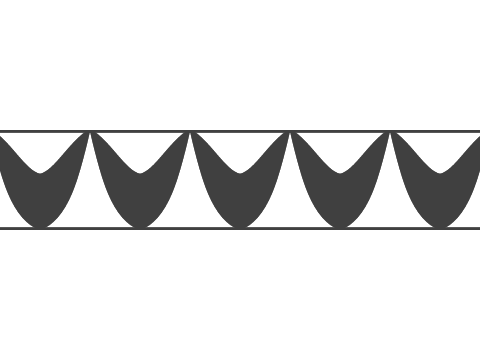
\includegraphics[width=.6\textwidth]{ansFv.png}
      \end{center}
    \end{enumerate}
  \end{freeResponse}
\end{question}
\mynewpage



\begin{question}
  Let's see what happens when we combine horizontal-reflections with
  other symmetries.
  \begin{enumerate}
  \item Can you find a frieze pattern that has symmetry through
    glide-reflections and $180^\circ$ rotations but not through
    horizontal-reflections? If YES, show me such a frieze pattern. If
    NO, explain why not.
  \item Can you find a frieze pattern that has symmetry through
    glide-reflections and horizontal-reflections but not through
    $180^\circ$ rotations? If YES, show me such a frieze pattern. If
    NO, explain why not.
  \end{enumerate}
    
  \begin{freeResponse}
    \begin{enumerate}
    \item NO, this cannot be done.
      \begin{itemize}
      \item First think about symmetry through glide-reflections. This
        means that the frieze pattern, when turned upside down, is a
        mirror image of itself.
      \item Next think about the $180^\circ$ rotation. This means that
        the frieze pattern, when turned upside down is unchanged.
      \end{itemize}
      This means that this frieze pattern is it's own mirror image. This
      means that the frieze pattern must have symmetry through
      horizontal-reflections.
    \item NO, this cannot be done.
      \begin{itemize}
      \item First think about symmetry through glide-reflections. This
        means that the frieze pattern, when turned upside down, is a
        mirror image of itself.
      \item Next think about the horizontal-reflection. This means
        that the frieze pattern is it's own mirror image.
      \end{itemize}
      This means that this frieze pattern is it's own mirror image
      when it is upside down, and hence must have symmetry through
      $180^\circ$ rotations.
    \end{enumerate}
  \end{freeResponse}
\end{question}
\mynewpage



\begin{question}
  DISPLAY a SINGLE frieze pattern that has symmetry through
  \begin{itemize}
  \item translations,
  \item glide-reflections,
  \item vertical-reflections,
  \item $180^\circ$ rotations, and
  \item horizontal-reflections.
  \end{itemize}
  \begin{freeResponse}
    Here it is:
    \begin{center}
      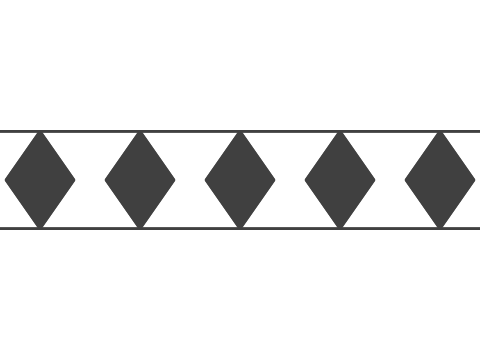
\includegraphics[width=.6\textwidth]{ansTGV8H.png}
    \end{center}
  \end{freeResponse}
\end{question}





\end{document}
